\chapter{结构之法}

这一章是关于字符串和链表的一些算法,也是面试中常考的数据结构。

这里我们先给出链表节点的定义。

\begin{Codex}[label={ListNode.java}]
class ListNode {
	public int data;
	public ListNode next;
	
	public ListNode(int x) {
		data = x;
		next = null;
	}
}
\end{Codex}

此外,本章还涉及到一些二叉树的算法,这里也先给出二叉树节点的定义。
\begin{Codex}[label={TreeNode.java}]
class TreeNode {
	public int data;
	public ListNode left, right;
	
	public TreeNode(int x) {
		data = x;
		left = right = null;
	}
}
\end{Codex}


% ----------------------------------------------------------------------------------------------------------------------------------------------------------------------
% ----------------------------------------------------------------------------------------------------------------------------------------------------------------------
% ----------------------------------------------------------------------------------------------------------------------------------------------------------------------
\section{字符串移位包含的问题} %%%%%%%%%%%%%%%%%%%%%%%%%%%%%%
\label{sec:string-shift-search}


\subsubsection{问题}
给定两个字符串$S_1$和$S_2$,要求判定$S_2$是否能够被$S_1$做循环移位(rotate)得到的字符串包含。例如,给定$S_1=AABCD$和$S_2=CDAA$,返回true,给定$S_1=ABCD$和$S_2=ACBD$,返回false。


\subsubsection{解法一}
对$S_1$做循环移位的操作等同于字符串连接操作$S_1S_1$,如果满足$|S_1|\geq|S_2|$和$S_2\subset S_1S_1$,那么$S_2$可以由$S_1$循环移位所得。时间复杂度为$O(N)$,其中$N=|S_1|$。

\begin{center}
	\Large
	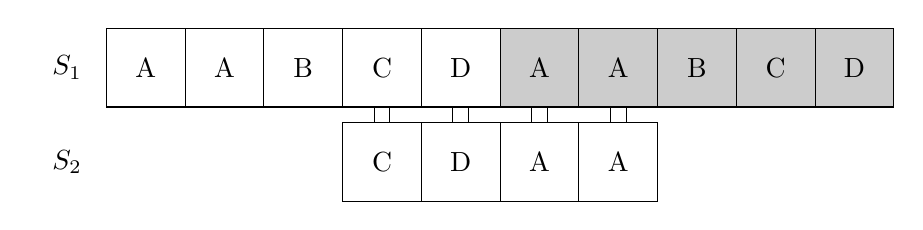
\begin{tikzpicture}[minimum size = 1cm]
	\node at (0,0) [rectangle] {$S_1$};
	\node at (1,0) [rectangle,draw] {A};
	\node at (2,0) [rectangle,draw] {A};
	\node at (3,0) [rectangle,draw] {B};
	\node at (4,0) [rectangle,draw] {C};
	\node at (5,0) [rectangle,draw] {D};
	\node at (6,0) [rectangle,draw=black, fill=black!20] {A};
	\node at (7,0) [rectangle,draw=black, fill=black!20] {A};
	\node at (8,0) [rectangle,draw=black, fill=black!20] {B};
	\node at (9,0) [rectangle,draw=black, fill=black!20] {C};
	\node at (10,0) [rectangle,draw=black, fill=black!20] {D};
	\node at (0,-1.2) [rectangle] {$S_2$};
	\node at (4,-1.2) [rectangle,draw] {C};
	\node at (5,-1.2) [rectangle,draw] {D};
	\node at (6,-1.2) [rectangle,draw] {A};
	\node at (7,-1.2) [rectangle,draw] {A};
	\draw (3.9,-0.5) -- (3.9, -0.7); \draw (4.1,-0.5) -- (4.1, -0.7);
	\draw (4.9,-0.5) -- (4.9, -0.7); \draw (5.1,-0.5) -- (5.1, -0.7);
	\draw (5.9,-0.5) -- (5.9, -0.7); \draw (6.1,-0.5) -- (6.1, -0.7);
	\draw (6.9,-0.5) -- (6.9, -0.7); \draw (7.1,-0.5) -- (7.1, -0.7);
	\end{tikzpicture}
	\figcaption{循环移位}\label{fig:string-shift-search-1}
\end{center}

\begin{Codex}[label={[$O(N)+O(N)$]Chap03_01_StringShiftSearch.java}]
boolean shiftSearch(String source, String target) {
	if (source.length() < target.length()) {
		return false;
	}
	source += source;
	// 也可以直接调用 return source.contains(target);
	return search(source, target);
}
// 这里也给出了字符串查找的代码,复杂度O(m*n)。
boolean search(String source, String target) {
	if (source.length() < target.length()) {
		return false;
	}
	int j = 0;
	for (int i = 0; i < source.length() && j < target.length(); i++) {
		if (source.charAt(i) == target.charAt(j)) {
			j++;
		} else {
			i -= j;
			j = 0;
		}
	}
	return j >= target.length();
}
\end{Codex}

\subsubsection{解法二}
解法一中申请了新的空间,其实是不必要的,我们可以通过直接操作$S_1$的下标$i$,使得$0\leq i \leq 2*|S_1|-1$,这样问题就变成了简单的字符串查找问题了。

\begin{Codex}[label={[$O(N)+O(1)$]Chap03_01_StringShiftSearch.java}]
boolean shiftSearch_2(String source, String target) {
	if (source.length() < target.length()) {
		return false;
	}
	int sLen = source.length();
	int tLen = target.length();
	int j = 0;
	for (int i = 0; i < sLen * 2 && j < tLen; i++) {
		if (source.charAt(i % sLen) == target.charAt(j)) {
			j++;
		} else {
			i -= j;
			j = 0;
		}
	}
	return j >= tLen;
}
\end{Codex}

% ----------------------------------------------------------------------------------------------------------------------------------------------------------------------
% ----------------------------------------------------------------------------------------------------------------------------------------------------------------------
% ----------------------------------------------------------------------------------------------------------------------------------------------------------------------
\section{电话号码对应英文单词} %%%%%%%%%%%%%%%%%%%%%%%%%%%%%%
\label{sec:phone-number}


\subsubsection{问题}
电话的号码盘一般可以用于输入字母,比如用2可以输入A,B,C,用3可以是如D,E,F,对于号码5869872,可以依次输出其代表的所有字母组合,如JTMWTPA……

\subsubsection{解法一}
利用递归,找出所有组合。

\begin{Codex}[label={[$O(3^N)+O(3^N)$]Chap03_02_PhoneNumber.java}]
public static final String[] maps = {"", "", "ABC", "DEF",
									 "GHI", "JKL", "MNO",
		 							 "PQRS", "TUV", "WXYZ"};

List<String> findWords(String phoneNumber) {
	List<String> words = new ArrayList<String>();
	words.add("");
	words = dfs(words, phoneNumber, 0);
	return words;
}

private List<String> dfs(List<String> words, String phoneNumber, int start) {
	if (start >= phoneNumber.length()) {
		return words;
	}
	List<String> list = new ArrayList<String>();
	int number = phoneNumber.charAt(start) - '0';
	for (String word : words) {
		for (int j = 0; j < maps[number].length(); j++) {
			list.add(word + maps[number].charAt(j));
		}
	}
	return dfs(list, phoneNumber, start + 1);
}
\end{Codex}

\subsubsection{解法二}
非递归版本。

\begin{Codex}[label={[$O(3^N)+O(3^N)$]Chap03_02_PhoneNumber.java}]
public static final String[] maps = {"", "", "ABC", "DEF",
									"GHI", "JKL", "MNO",
									"PQRS", "TUV", "WXYZ"};
	
List<String> findWords_2(String phoneNumber) {
	List<String> words = new ArrayList<String>();
	words.add("");
	for (int i = 0; i < phoneNumber.length(); i++) {
		List<String> list = new ArrayList<String>();
		for (String word : words) {
			int number = phoneNumber.charAt(i) - '0';
			for (int j = 0; j < maps[number].length(); j++) {
				list.add(word + maps[number].charAt(j));
			}
		}
		words = list;
	}
	return words;
}
\end{Codex}

% ----------------------------------------------------------------------------------------------------------------------------------------------------------------------
% ----------------------------------------------------------------------------------------------------------------------------------------------------------------------
% ----------------------------------------------------------------------------------------------------------------------------------------------------------------------
\section{计算字符串的相似度} %%%%%%%%%%%%%%%%%%%%%%%%%%%%%%
\label{sec:string-similarity}


\subsubsection{问题}
字符串之间的相似度等于“距离+1”的倒数,而字符串之间的距离定义为将一个字符串变换到另一个字符串的操作次数。这里我们定义了三种操作:

\subsubsection{解法一}
算法时间复杂度为$O(N*M)$,其中$N=|S|,M=|T|$。

\begin{Codex}[label={[$O(N*M)+O(N*M)$]Chap03_03_StringSimilarity.java}]
int similarity(String s, String t) {
	s = "$" + s;
	t = "$" + t;
	int sLen = s.length();
	int tLen = t.length();
	int[][] dist = new int[sLen][tLen];
	for (int i = 0; i < tLen; i++) {
		dist[0][i] = i;
	}
	for (int i = 0; i < sLen; i++) {
		dist[i][0] = i;
	}
	for (int i = 1; i < sLen; i++) {
		for (int j = 1; j < tLen; j++) {
			dist[i][j] = dist[i - 1][j - 1]
					+ (s.charAt(i) == t.charAt(j) ? 0 : 1);
			dist[i][j] = Math.min(dist[i][j],
					Math.min(dist[i - 1][j], dist[i][j - 1]) + 1);
		}
	}
	return dist[sLen - 1][tLen - 1];
}
\end{Codex}


\subsubsection{解法二}
可以采用滚动数组来节省空间。

\begin{Codex}[label={[$O(N*M)+O(M)$]Chap03_03_StringSimilarity.java}]
int similarity(String s, String t) {
	s = "$" + s;
	t = "$" + t;
	int sLen = s.length();
	int tLen = t.length();
	int[][] dist = new int[2][tLen];
	for (int i = 0; i < tLen; i++) {
		dist[0][i] = i;
	}
	dist[1][0] = 1;
	for (int i = 1; i < sLen; i++) {
		for (int j = 1; j < tLen; j++) {
			dist[i % 2][j] = dist[(i + 1) % 2][j - 1]
					+ (s.charAt(i) == t.charAt(j) ? 0 : 1);
			dist[i % 2][j] = Math.min(dist[i % 2][j],
					Math.min(dist[(i + 1) % 2][j], dist[i % 2][j - 1]) + 1);
		}
	}
	return dist[(sLen + 1) % 2][tLen - 1];
}
\end{Codex}

% ----------------------------------------------------------------------------------------------------------------------------------------------------------------------
% ----------------------------------------------------------------------------------------------------------------------------------------------------------------------
% ----------------------------------------------------------------------------------------------------------------------------------------------------------------------
\section{从无头单链表中删除节点} %%%%%%%%%%%%%%%%%%%%%%%%%%%%%%
\label{sec:delete-linked-list-node}


\subsubsection{问题}
假设有一个没有头指针的单链表,一个指针指向此单链表中间的一个节点(不是第一个,也不是最后一个),请将该节点从单链表中删除。

\subsubsection{解法}

\begin{Codex}[label={[$O(1)+O(1)$]Chap03_04_DeleteLinkedListNode.java}]
void deleteNode(ListNode p) {
	if (p.next == null) {
		return;
	}
	p.data = p.next.data;
	p.next = p.next.next;
}
\end{Codex}

% ----------------------------------------------------------------------------------------------------------------------------------------------------------------------
% ----------------------------------------------------------------------------------------------------------------------------------------------------------------------
% ----------------------------------------------------------------------------------------------------------------------------------------------------------------------
\section{编程判断两个链表是否相交} %%%%%%%%%%%%%%%%%%%%%%%%%%%%%%
\label{sec:linkedlist-intersection}


\subsubsection{问题}
给出两个单向链表的头指针,判断这两个链表是否相交。这里假设两个链表均不带环。

\subsubsection{解法}
如果两个链表相交,那么这两个链表的最后一个指针一定是相同的。因此我们只要记录下两个链表最后一个指针$A_{tail}$和$B_{tail}$,判断它们是否相同即可。

\begin{Codex}[label={[$O(L)+O(0)$]Chap03_06_LinkedListIntersection.java}]
boolean isIntersection(ListNode headA, ListNode headB) {
	if (headA == null || headB == null) {
		return false;
	}
	while (headA.next != null) {
		headA = headA.next;
	}
	while (headB.next != null) {
		headB = headB.next;
	}
	return headA == headB;
}
\end{Codex}

\subsubsection{扩展问题}
如何求出这两个链表相交的第一个节点呢?

\subsubsection{解法}
既然相交,那么最后一个节点一定相同,然后就去判断倒数第二个节点是否相同,以此类推。现在的问题就是这是单向链表,所以只能从头向后遍历,因此我们可以先让两个链表的长度变成一样的,就是遍历那个长的链表直到长度和短链表相同。
然后,这时候就可以同时遍历这两个链表并判断节点是否相同,若相同则返回。直到遍历到链表的结尾,一定会有一个节点返回(因为最后一个节点一定是相同的)。

\begin{Codex}[label={[$O(L)+O(1)$]Chap03_06_LinkedListIntersection.java}]
ListNode findIntersection(ListNode headA, ListNode headB) {
	int lenA = lengthOfLinkedList(headA);
	int lenB = lengthOfLinkedList(headB);
	while (lenA >= 0) {
		if (headA == headB) {
			return headA;
		}
		int diff = lenA - lenB;
		if (diff >= 0) {
			lenA--;
			headA = headA.next;
		}
		if (diff <= 0) {
			lenB--;
			headB = headB.next;
		}
	}
	return null;
}
// 计算链表长度
int lengthOfLinkedList(ListNode head) {
	int length = 0;
	while (head != null) {
		length++;
		head = head.next;
	}
	return length;
}
\end{Codex}

% ----------------------------------------------------------------------------------------------------------------------------------------------------------------------
% ----------------------------------------------------------------------------------------------------------------------------------------------------------------------
% ----------------------------------------------------------------------------------------------------------------------------------------------------------------------
\section{队列中取最大值操作问题} %%%%%%%%%%%%%%%%%%%%%%%%%%%%%%
\label{sec:max-queue}


\subsubsection{问题}
假设有这样一个拥有3个操作的队列:
\begin{enumerate}
	\item EnQueue(v): 将v加入队列中。
	\item DeQueue: 删除队首元素并返回。
	\item MaxElement: 返回队列中的最大元素。
\end{enumerate}

请设计一种数据结构和算法,让MaxElement操作的时间复杂度尽可能的降低。

\subsubsection{解法}
增加一个max数组表示队列中最大元素,对于入队操作,如果元素v比max数组最后一个元素大,就删除max最后一个元素,将v加入到max数组中。反之,如果v小于max最后一个元素,就直接将v加入到max数组中。
对于出队操作,如果出队元素和max数组第一个元素相同,就删除max第一个元素。

\begin{Codex}[label={[$O(1)+O(N)$]Chap03_07_MaxQueue.java}]
public class MaxQueue {
	Queue<Integer> queue = new LinkedList<Integer>();
	List<Integer> max = new LinkedList<Integer>();
	void push(int x) {
		queue.offer(x);
		if(max.size()==0 || x<=max.get(max.size()-1)) {
			max.add(x);
		} else {
			max.remove(max.size()-1);
			max.add(x);
		}
	}
	int pop() {
		int x = queue.poll();
		if(x==max.get(0)) {
			max.remove(0);
		}
		return x;
	}
	int maxElement() {
		return max.get(0);
	}
}
\end{Codex}

% ----------------------------------------------------------------------------------------------------------------------------------------------------------------------
% ----------------------------------------------------------------------------------------------------------------------------------------------------------------------
% ----------------------------------------------------------------------------------------------------------------------------------------------------------------------
\section{求二叉树中节点的最大距离} %%%%%%%%%%%%%%%%%%%%%%%%%%%%%%
\label{sec:max-dist-in-binary-tree}


\subsubsection{问题}
我们定义二叉树中两个节点的距离为两个节点之间边的个数。求一棵二叉树中相距最远的两个节点之间的距离。

\subsubsection{解法}
我们先来定义经过节点$R$的最大距离为$f(R)$,那么整棵树的最大距离就是$f(T)=max_{R\in T}{f(R)}$。
所以我们只要求出每个节点的$f(R)$即可,我们会发现经过节点$R$的最大距离的两个节点一定分别来自左右两个子树(或者树根$R$),并且一定是距离$R$最远的两个叶子节点。

所以我们推出下面的公式:
\[
f(R) = H(R_{left}) + H(R_{right}) + 1
\]
其中$H(R)$是以$R$为树根的子树的高度。

\begin{Codex}[label={[$O(N)+O(1)$]Chap03_08_MaxDistInBinaryTree.java}]
int ans = 1;

public int maxDist(TreeNode root) {
	maxHeight(root);
	return ans - 1;
}

public int maxHeight(TreeNode root) {
	if (root == null) {
		return 0;
	}
	int leftDist = maxHeight(root.left);
	int rightDist = maxHeight(root.right);
	ans = Math.max(ans, leftDist + rightDist + 1);
	return Math.max(leftDist, rightDist) + 1;
}
\end{Codex}


% ----------------------------------------------------------------------------------------------------------------------------------------------------------------------
% ----------------------------------------------------------------------------------------------------------------------------------------------------------------------
% ----------------------------------------------------------------------------------------------------------------------------------------------------------------------
\section{重建二叉树} %%%%%%%%%%%%%%%%%%%%%%%%%%%%%%
\label{sec:construct-binary-tree}


\subsubsection{问题}
给出二叉树的前序遍历和中序遍历的结果,求出原始的二叉树。

\subsubsection{解法}
前序遍历结果为:$[a,b,d,c,e,f]$,

中序遍历结果为:$[d,b,a,e,c,f]$。

构造出的二叉树如图所示:

\begin{center}
	\Large
	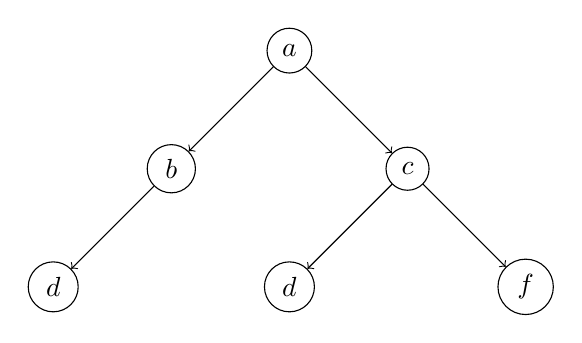
\begin{tikzpicture}
	\node (d) at (0,0) [circle, draw] {$d$};
	\node (b) at (1.5,1.5) [circle, draw] {$b$} edge [->] (d);
	\node (e) at (3,0) [circle, draw] {$d$};
	\node (f) at (6,0) [circle, draw] {$f$};
	\node (c) at (4.5,1.5) [circle, draw] {$c$} edge [->] (e) edge [->] (f);
	\node (a) at (3,3) [circle, draw] {$a$} edge [->] (b) edge [->] (c);
	\end{tikzpicture}
	\figcaption{重建二叉树}\label{fig:construct-binary-tree-1}
\end{center}

对于前序遍历$[\underline{a},b,d,c,e,f]$中$\underline{a}$一定是根节点,因此我们在中序遍历$[d,b,\underline{a},e,c,f]$中也找到$\underline{a}$,根据中序遍历可以知道$[d,b]$是左子树,$[e,c,f]$是右子树。
从而可以递归构造左子树并返回左子树的根节点作为当前节点的左孩子,同理构造右子树。

\begin{Codex}[label={[$O(N)+O(1)$]Chap03_09_ConstructBinaryTree.java}]
public TreeNode buildTree(String preorder, String inorder) {
	if (preorder == null) {
		return null;
	}
	char val = preorder.charAt(0);
	TreeNode node = new TreeNode(val);
	int idx = inorder.indexOf(val);
	if (idx > 0) {
		node.left = buildTree(preorder.substring(1, idx + 1), inorder.substring(0, idx));
	}
	if (idx < inorder.length() - 1) {
		node.right = buildTree(preorder.substring(idx + 1), inorder.substring(idx + 1));
	}
	return node;
}
\end{Codex}


% ----------------------------------------------------------------------------------------------------------------------------------------------------------------------
% ----------------------------------------------------------------------------------------------------------------------------------------------------------------------
% ----------------------------------------------------------------------------------------------------------------------------------------------------------------------
\section{分层遍历二叉树} %%%%%%%%%%%%%%%%%%%%%%%%%%%%%%
\label{sec:tree-level-order-traversal}


\subsubsection{问题}
分层输出二叉树的节点。
\begin{center}
	\Large
	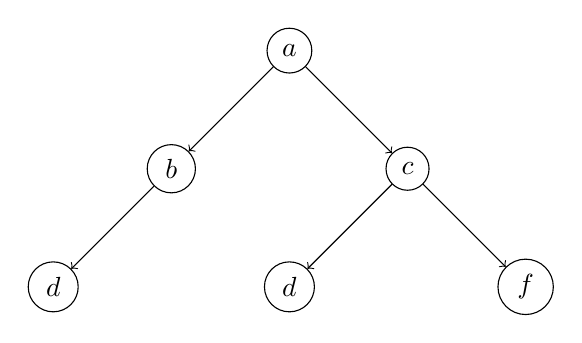
\begin{tikzpicture}
	\node (d) at (0,0) [circle, draw] {$d$};
	\node (b) at (1.5,1.5) [circle, draw] {$b$} edge [->] (d);
	\node (e) at (3,0) [circle, draw] {$d$};
	\node (f) at (6,0) [circle, draw] {$f$};
	\node (c) at (4.5,1.5) [circle, draw] {$c$} edge [->] (e) edge [->] (f);
	\node (a) at (3,3) [circle, draw] {$a$} edge [->] (b) edge [->] (c);
	\end{tikzpicture}
	\figcaption{分层遍历二叉树}\label{fig:tree-level-order-traversal-1}
\end{center}
输出结果为:

a

b c

d e f

\subsubsection{解法}
利用队列。

\begin{Codex}[label={[$O(N)+O(N)$]Chap03_10_TreeLevelOrderTraversal.java}]
public void traversal(TreeNode root) {
	if (root == null) {
		return;
	}
	Queue<TreeNode> queue = new LinkedList<TreeNode>();
	queue.offer(root);
	int curLayer = 1;
	int nextLayer = 0;
	while (!queue.isEmpty()) {
		TreeNode node = queue.poll();
		curLayer--;
		System.out.printf("%d ", node.data);
		if (node.left != null) {
			queue.offer(node.left);
			nextLayer++;
		}
		if (node.right != null) {
			queue.offer(node.right);
			nextLayer++;
		}
		if (curLayer == 0) {
			System.out.println();
			curLayer = nextLayer;
			nextLayer = 0;
		}
	}
}
\end{Codex}

% ----------------------------------------------------------------------------------------------------------------------------------------------------------------------
% ----------------------------------------------------------------------------------------------------------------------------------------------------------------------
% ----------------------------------------------------------------------------------------------------------------------------------------------------------------------
\section{程序改错} %%%%%%%%%%%%%%%%%%%%%%%%%%%%%%
\label{sec:debug-code}


\subsubsection{问题}
找出一个有序数组A中等于目标值targe的元素的序号,如果有多个元素满足条件则返回序号最大的,如果没有则返回-1。

\subsubsection{解法}
二分查找。

\begin{Codex}[label={[$O(lg(N))+O(1)$]Chap03_11_DebugCode.java}]
int bsearch3(int[] A, int target) {
	int left = -1, right = A.length;
	while (right - left > 1) {
		int mid = (left + right) >>> 1;
		if (A[mid] <= target) {
			left = mid;
		} else {
			right = mid;
		}
	}
	if (A[left] == target) {
		return left;
	}
	return -1;
}
\end{Codex}